\documentclass[10pt]{beamer}

\usetheme{metropolis}
\definecolor{WiLabRed}{RGB}{197,18,48}
\setbeamercolor{frametitle}{fg=white,bg=WiLabRed}
\setbeamercolor{progress bar}{fg=WiLabRed!90}
\setbeamercolor{title separator}{fg=WiLabRed!90}
\setbeamercolor{progress bar in section page}{fg=WiLabRed!90}
\setbeamercolor{background canvas}{bg=white}
\setbeamercolor{alerted text}{fg=WiLabRed!90}

\usepackage{appendixnumberbeamer}

\usepackage{booktabs}
\usepackage[scale=2]{ccicons}

\usepackage{pgfplots}
\usepgfplotslibrary{dateplot}

\usepackage{xspace}
\newcommand{\themename}{\textbf{\textsc{metropolis}}\xspace}

\usepackage{marvosym}
%\usepackage{subfig}
\usepackage{graphicx}\graphicspath{{images/}}
%\usepackage{subcaption}
\usepackage[framed]{mcode}
\usepackage{listings}

\title{Laboratory 3: Frame Synchronization}
\subtitle{\textit{Software Defined Radio for Engineers} (Collins~\textit{et al.}), \textsection{8.1-8.2}}
\date{}
\author{\textbf{Alexander M. Wyglinski, Ph.D.}}
\institute{ \vspace*{1in}\hfill
\includegraphics[height=1.125cm]{wilab_logo-A70916.eps} \qquad 
\includegraphics[height=1.125cm]{WPI_Inst_Prim_FulClr.eps}}
% \titlegraphic{\hfill\includegraphics[height=1.5cm]{logo.pdf}}

% Foot for all slides
\setbeamertemplate{frame footer}{\tiny \copyright~2018 by Alexander Wyglinski. This work is licensed under the Creative Commons Attribution-ShareAlike 4.0 International License. To view a copy of this license, visit http://creativecommons.org/licenses/by-sa/4.0/.}

\begin{document}

%\captionsetup[subfigure]{labelformat=empty}

%%%%%%%%%%%%%%%%%%%%%%%%%%%%%%%%%%%%%%%%%%%%%%%%%%%%%%%%%%

\maketitle




%%%%%%%%%%%%%%%%%%%%%%%%%%%%%%%%%%%%%%%%%%%%%%%%%%%%%%%%%%

\frame
{
  \frametitle{Visual Representation of Unknown Signal}
    %\begin{itemize}
    \begin{figure}
  				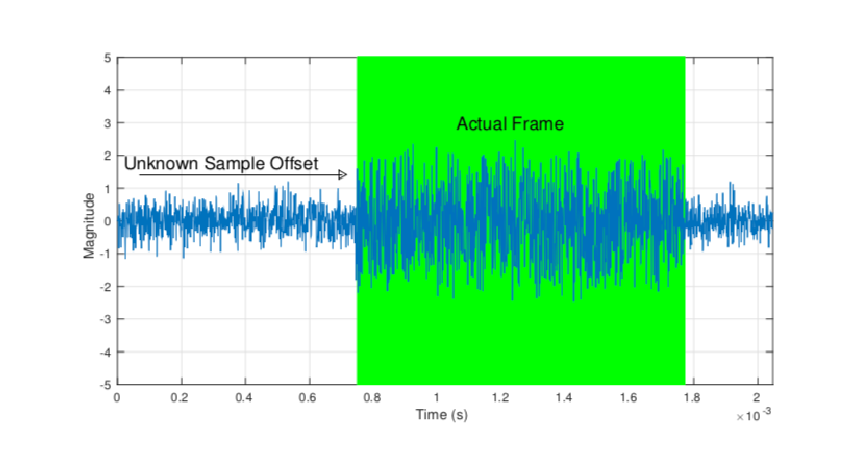
\includegraphics[width=\linewidth]{Delay.eps}
 				 \caption{Unknown Signal Delay}
  				\label{fig:Example received frame in AWGN with an unknown sample offset}
		\end{figure}
    %\end{itemize}

}

\frame
{
  \frametitle{Revisting Several Concepts}

    \begin{itemize}
        \item We have a delayed signal free of any offset errors
        \begin{equation}
        \begin{split}
            u[n]=y[n-p]
        \end{split}
        \end{equation}
        \hspace{5ex} where $p \in Z$
        \item To get to the start of the frame we will use barker codes 
         \item Aautocorrelation function of barker codes is given as:
        \begin{equation}
        \begin{split}
            C(k) = \sum_{i=1}^{N-k} a[i]a[i+k]
        \end{split}
        \end{equation}
        
    \end{itemize}
      \hspace{5ex} such that $|c(v)|\leq 1$ and $1\leq v \leq N$

}

\frame
{
  \frametitle{Barker Sequence Example}

    \begin{itemize}
        \item Consider a barker sequence $a[k]$ and data sequence $r[k]$
        \item We randomly insert $a[k]$ into $r[k]$ at random position $p$
        \item We apply cross-correlation will length $2L_r - 1$ 
        
        where $L_r$ is length of $r$
    \end{itemize}

}

\frame
{
  \frametitle{Barker Sequence Example}

    \begin{itemize}
        \item $a[k]$ will be padded with zeros such that the code lengths are equal 
        \item A peak will occur at $L_a$ samples from the start 
        \item The offset position for the sequence can then be determined using: 
         \begin{equation}
        \begin{split}
        \hat{p} = \arg\max c_{ra}[k]-L_r
        \end{split}
        \end{equation} 
    \end{itemize}

}
\frame
{
  \frametitle{Visual Output}
    %\begin{itemize}
    \begin{figure}
  				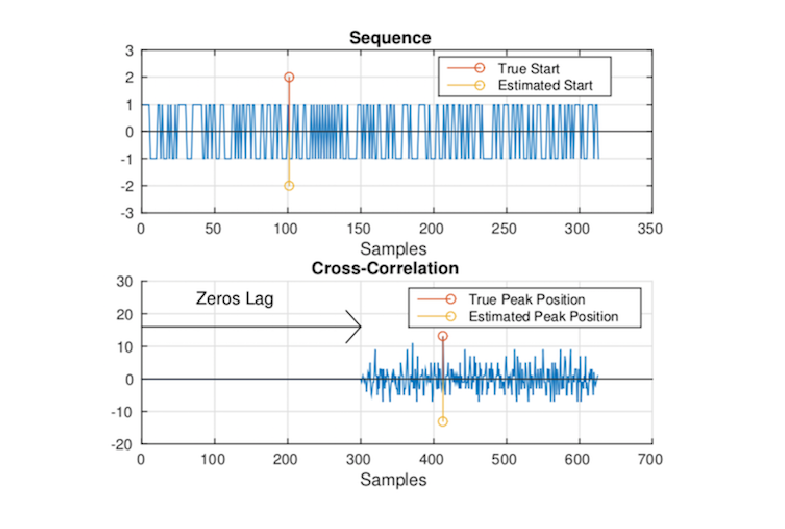
\includegraphics[width=0.8\linewidth, scale=0.5]{Output.eps}
 				 \caption{Offset Position}
  				\label{fig:Sample Barker Code implementation for sequence offset determination}
		\end{figure}
    %\end{itemize}

}

\frame
{
  \frametitle{Next Problem?}
    \begin{itemize}
    \item How do we know if the frame actually exist in the correlation?
    \item Detection becomes a thresholding problem 
    \item However, even without a frame peaks can appear larger
    \item We will access this in the second part of this laboratory experiment
    \end{itemize}

}

\frame
{
  \frametitle{Frame Detection Problems}
    %\begin{itemize}
    \begin{figure}
  				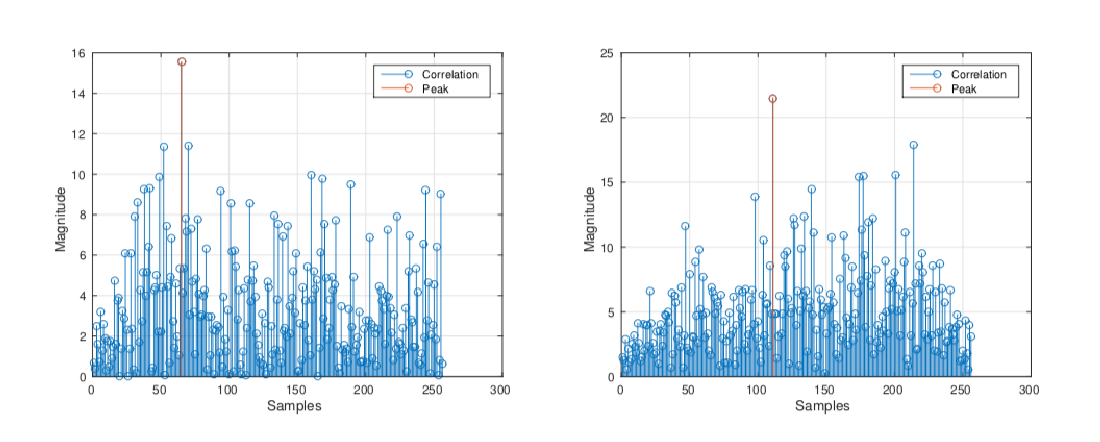
\includegraphics[width=\linewidth, scale=0.5]{Problem.eps}
 				 \caption{Frame Detection}
  				\label{fig:Correlation with and without signal being present}
		\end{figure}
    %\end{itemize}

}





\end{document}
